\documentclass[report]{../../custom}
\begin{document}
\maketitle

\noindent \textbf{摘要:}
本周主要完成了自适应线程分配(ATA)方法的实验验证与扩展应用。通过对80种不同block和thread配置的系统性测试,成功建立了性能优化函数模型,将ATA从公钥生成扩展至签名过程。实验结果显示,我们的方法在签名性能上实现了17.4\%的提升(从0.0605降至0.0493)。同时,完成了包含自适应线程分配和函数级并行两个核心组件的优化架构图设计,为论文框架提供了清晰的视觉表达。
\vskip 0.5cm

\noindent \textbf{下周计划:}
1) 开始论文实验章节书写;
2) 完善创新点2,函数级并行优化

\section{论文实验}

本周我们将上周提出的自适应线程函数进行实验验证,其中我们将其从公钥的生成扩展到签名过程,并在此基础上进行性能分析。

\subsection{线程数与性能}

实验系统性测试了8种不同block数量(32至256)和10种不同thread数量(64至512),共80种配置组合对密钥生成和签名操作的影响。如图\ref{fig:thread_time_cost}所示。通过对实验数据进行函数拟合,我们得到了图\ref{fig:approach}中的性能预测曲线。该模型成功预测出最优线程配置,与实际性能测量高度吻合,证实了我们方法的有效性。与\cite{Wang2025}的基准实现相比,我们在签名处理时间上从0.0605秒降至0.0493秒,实现了17.4\%的性能提升。

\begin{figure}[h]
  \centering
  \begin{subfigure}{0.48\textwidth}
    \centering
    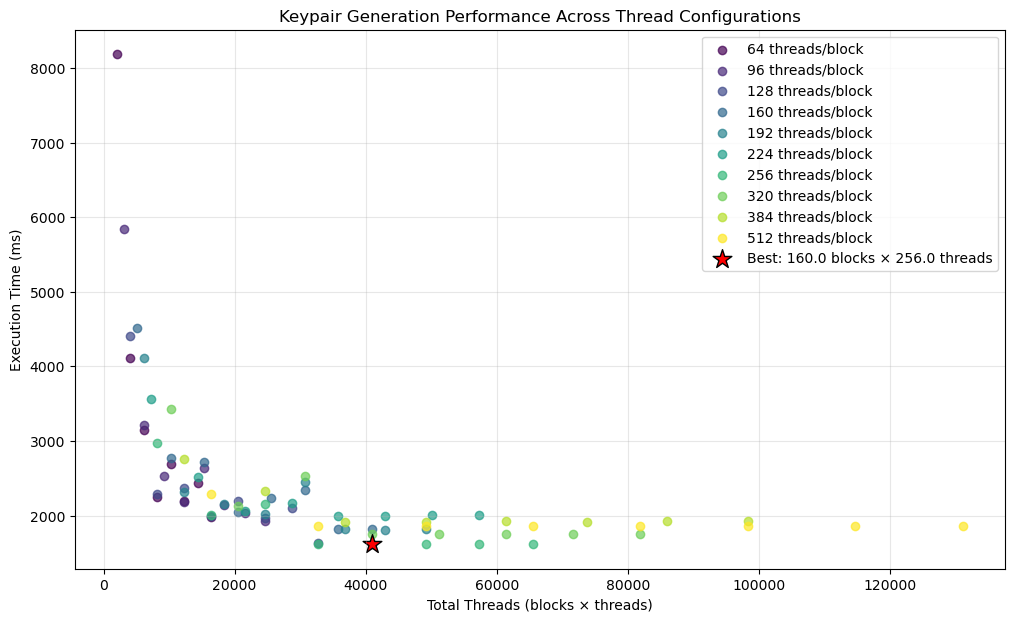
\includegraphics[width=\textwidth]{./fig/thread_time_cost.png}
    \caption{不同block和thread配置下的性能对比}
    \label{fig:thread_time_cost}
  \end{subfigure}
  \hfill
  \begin{subfigure}{0.48\textwidth}
    \centering
    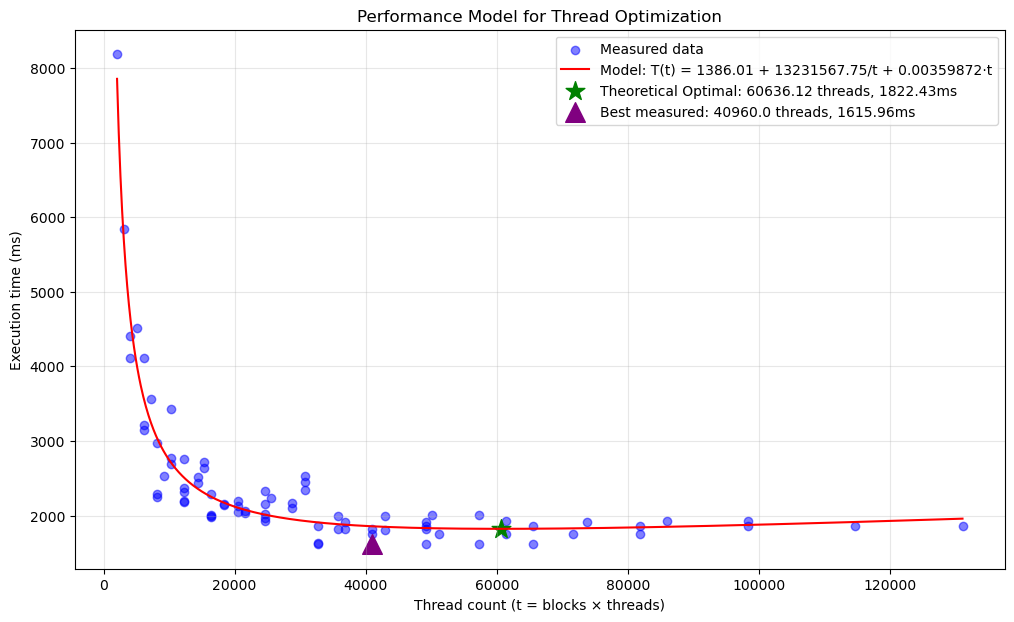
\includegraphics[width=\textwidth]{./fig/approach.png}
    \caption{性能函数拟合曲线}
    \label{fig:approach}
  \end{subfigure}
  \caption{线程配置性能分析}
  \label{fig:performance}
\end{figure}

\subsection{thread和block的选择}

我们进一步分析了在固定总并行度条件下,block和thread分配比例对性能的影响。图\ref{fig:block_thread_time}展示了不同配置组合的性能对比。数据表明,当每个block包含256个threads时,签名和公钥生成操作均达到最佳性能。这一发现具有显著实用价值,因为它表明在我们的SPHINCS+实现中存在一个明确的线程组织最优点,该配置能够最有效地平衡线程管理开销与并行计算效率。我们推测这与GPU内存层次结构和warp执行模式的交互有关,将在论文中进行分析。

\begin{figure}
  \centering
  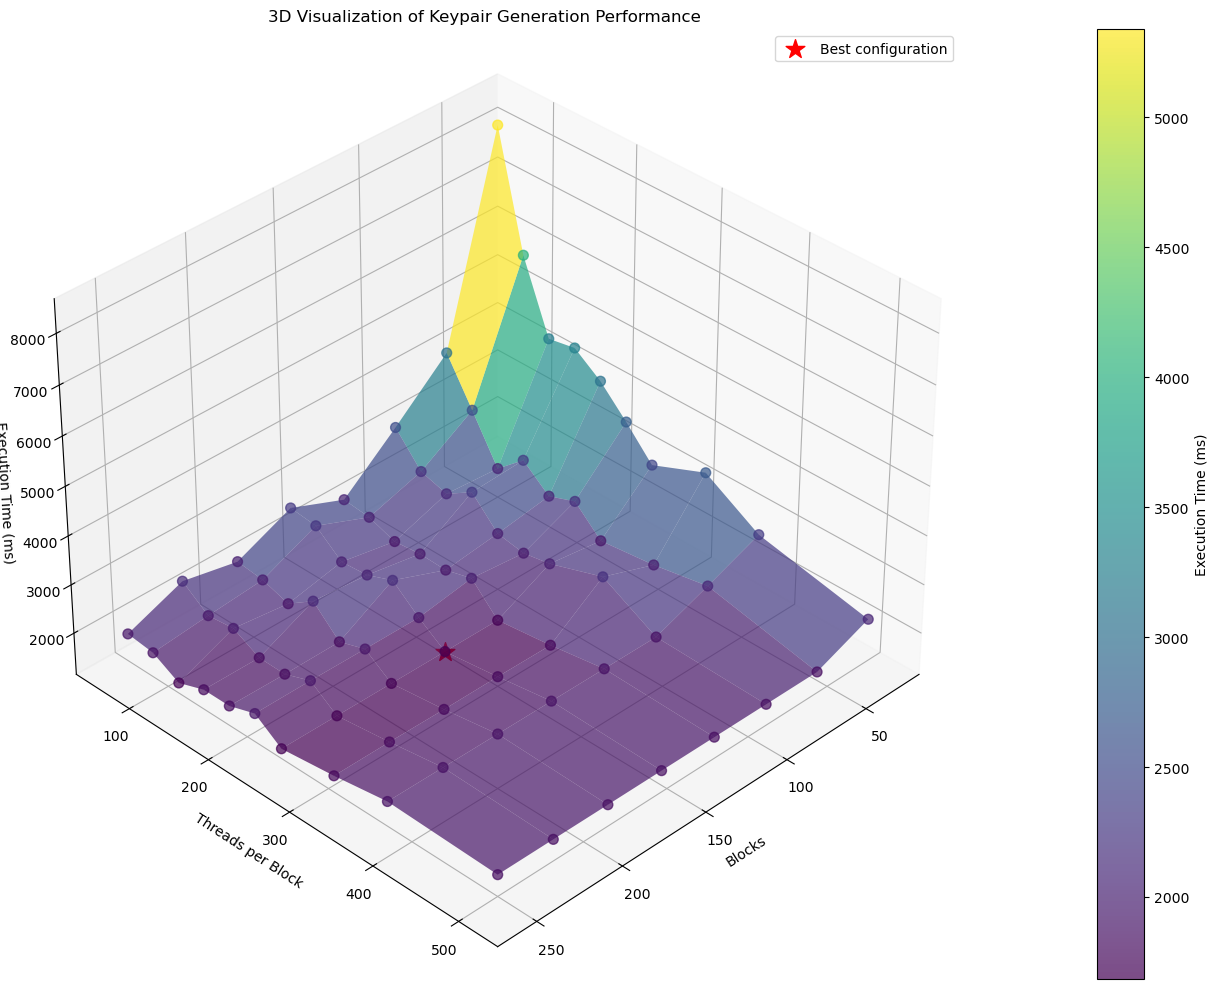
\includegraphics[width=0.5\textwidth]{./fig/block_thread_time.png}
  \caption{不同block和thread配置下的性能对比}
  \label{fig:block_thread_time}
\end{figure}

\section{论文写作}

\subsection{优化架构图}

设计并完成了优化框架的整体架构图(图\ref{fig:optimization_architecture})。该图展示了我们提出的双组件优化架构:自适应线程分配(Adaptive Thread Allocation, ATA)和函数级并行(Function-Level Parallelism, FLP)。ATA组件负责动态确定最优的GPU线程配置,而FLP组件则实现算法中不同函数的并行执行。这种层次化优化策略能够在不同级别上提升计算效率,显著优于单一优化方法。该架构图将作为论文的核心图表之一,有助于清晰传达我们的方法论。

\begin{figure}
  \centering
  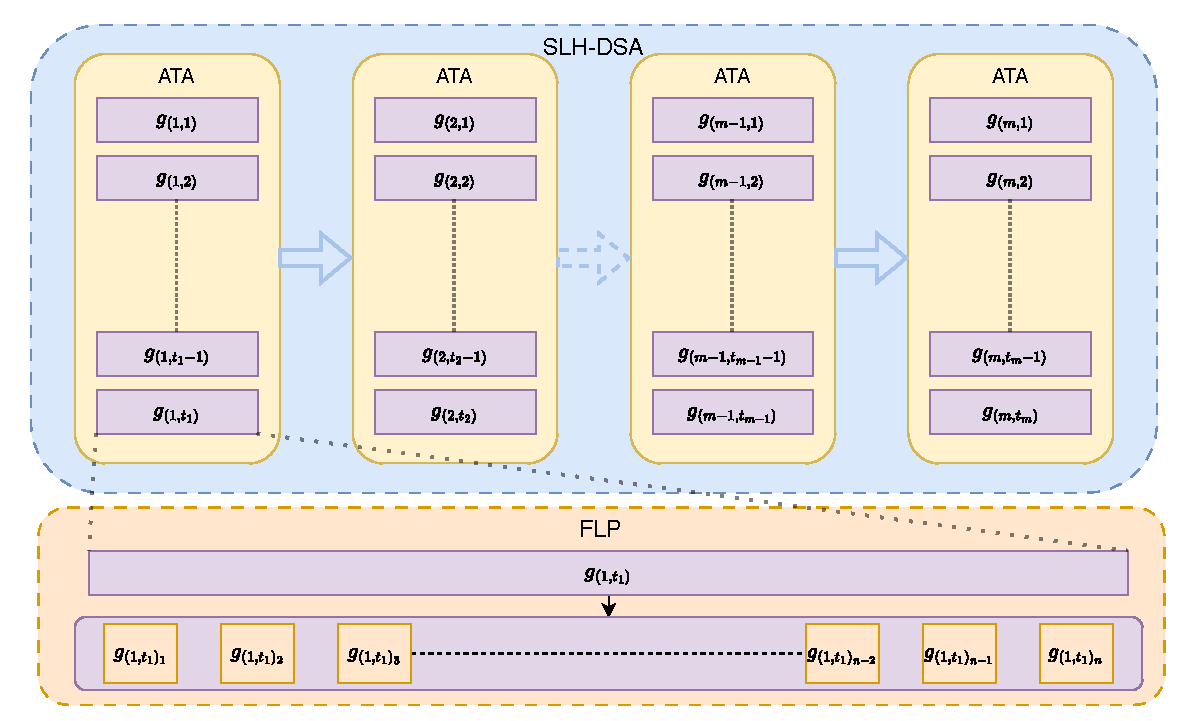
\includegraphics[width=0.5\textwidth]{./fig/optimize-overview.pdf}
  \caption{优化架构图}
  \label{fig:optimization_architecture}
\end{figure}

\bibliographystyle{alpha}
\bibliography{../../paper}

\end{document}